% edit & compile online at https://letx.app
\documentclass[11pt,aspectratio=169]{beamer}
\usetheme{default}

% Packages for styling and layout
\usepackage[utf8]{inputenc}
\usepackage[T1]{fontenc}
\usepackage{lato}
\renewcommand{\familydefault}{\sfdefault}
\usepackage{booktabs}
\usepackage{pgfplots}
\pgfplotsset{compat=1.17}
\usepackage{amsmath}
\usepackage{amssymb}
\usepackage{microtype}
\usepackage{tikz}

% Colors
\definecolor{cosmicnavy}{RGB}{12, 24, 48}      % Deep space navy (primary)
\definecolor{cosmicslate}{RGB}{86, 108, 129}   % Slate grey-blue (secondary)
\definecolor{cosmicgold}{RGB}{197, 143, 45}    % Warm gold (accent)
\definecolor{cosmicbg}{RGB}{252, 252, 252}     % Pure light off-white (bg)
\definecolor{cosmiccharcoal}{RGB}{43, 45, 48}  % Body text charcoal
\definecolor{cosmiclight}{RGB}{242, 244, 247}   % Light block background

% Set Beamer Colors
\setbeamercolor{background canvas}{bg=cosmicbg}
\setbeamercolor{normal text}{fg=cosmiccharcoal}
\setbeamercolor{structure}{fg=cosmicnavy}
\setbeamercolor{title}{fg=cosmicnavy}
\setbeamercolor{subtitle}{fg=cosmicslate}
\setbeamercolor{frametitle}{fg=cosmicnavy}
\setbeamercolor{framesubtitle}{fg=cosmicslate}
\setbeamercolor{item}{fg=cosmicslate}
\setbeamercolor{subitem}{fg=cosmicslate}
\setbeamercolor{alerted text}{fg=cosmicgold}
\setbeamercolor{block title}{fg=white, bg=cosmicnavy}
\setbeamercolor{block body}{fg=cosmiccharcoal, bg=cosmiclight}

% Fonts
\setbeamerfont{title}{size=\LARGE, series=\bfseries}
\setbeamerfont{subtitle}{size=\large, series=\normalfont}
\setbeamerfont{frametitle}{size=\large, series=\bfseries}
\setbeamerfont{framesubtitle}{size=\small, series=\normalfont}
\setbeamerfont{section title}{size=\huge, series=\bfseries}
\setbeamerfont{author}{size=\normalsize}
\setbeamerfont{institute}{size=\scriptsize}
\setbeamerfont{date}{size=\scriptsize}

% Layout and Templates
\setbeamertemplate{navigation symbols}{}
\setbeamertemplate{blocks}[rounded=false, shadow=false]

% Clean itemize bullets
\setbeamertemplate{itemize item}{\raise0.3ex\hbox{\fontsize{5pt}{5pt}\selectfont$\bullet$}}
\setbeamertemplate{itemize subitem}{\raise0.3ex\hbox{\fontsize{4pt}{4pt}\selectfont$\circ$}}

% Footline
\setbeamertemplate{footline}{
  \ifnum\insertframenumber>1
    \begin{beamercolorbox}[wd=\paperwidth,ht=3ex,dp=2ex,leftskip=1cm,rightskip=1cm]{footline}
      \fontsize{7pt}{9pt}\selectfont
      \textcolor{cosmicslate}{\rule{\dimexpr\paperwidth-2cm\relax}{0.3pt}} \\ \vspace{0.5ex}
      \textcolor{cosmicslate}{Dr. Elena Vance (IGP)} \hfill 
      \textcolor{cosmicslate}{GW Standard Sirens \& the Hubble Tension} \hfill 
      \textcolor{cosmicslate}{\insertframenumber\,/\,\inserttotalframenumber}
    \end{beamercolorbox}
  \fi
}

% Title Page Template
\setbeamertemplate{title page}{
  \vbox{}
  \vfill
  \begin{flushleft}
    {\color{cosmicgold}\rule{1.5cm}{1.5pt}}\par\vspace{0.4cm}
    {\usebeamerfont{title}\usebeamercolor[fg]{title}\inserttitle}\par
    \ifx\insertsubtitle\empty\else
      \vspace{0.2cm}
      {\usebeamerfont{subtitle}\usebeamercolor[fg]{subtitle}\insertsubtitle}\par
    \fi
    \vspace{1.2cm}
    {\usebeamerfont{author}\insertauthor}\par
    \vspace{0.1cm}
    {\usebeamerfont{institute}\insertinstitute}\par
    \vspace{0.5cm}
    {\usebeamerfont{date}\insertdate}\par
  \end{flushleft}
  \vfill
}

% Section Divider Template
\setbeamertemplate{section page}{
  \vbox{}
  \vfill
  \begin{flushleft}
    {\color{cosmicgold}\rule{1.2cm}{1.2pt}}\par\vspace{0.4cm}
    {\usebeamerfont{section title}\usebeamercolor[fg]{title}\insertsection}\par
  \end{flushleft}
  \vfill
}
\AtBeginSection{
  \begin{frame}[plain,c]
    \sectionpage
  \end{frame}
}

% Presentation Metadata
\title{Gravitational-Wave Standard Sirens}
\subtitle{A New Window on the Hubble Tension}
\author{Dr. Elena Vance}
\institute{Institute for Gravitational Physics, Department of Astrophysics \\ Cosmic Cosmology Colloquium 2026}
\date{July 7, 2026}

\begin{document}

% Slide 1: Title Slide
\begin{frame}[plain]
  \titlepage
\end{frame}

% Slide 2: Outline
\begin{frame}{Talk Outline}
  \begin{columns}[T]
    \begin{column}{0.45\textwidth}
      \begin{itemize}
        \setlength{\itemsep}{1em}
        \item \textbf{The Hubble Tension}
        \begin{itemize}
          \item Early vs. Late Universe probes
          \item Systematics vs. New Physics
        \end{itemize}
        \item \textbf{Standard Sirens}
        \begin{itemize}
          \item Gravitational-wave distance calibration
          \item Absolute vs. relative measurements
        \end{itemize}
      \end{itemize}
    \end{column}
    \begin{column}{0.45\textwidth}
      \begin{itemize}
        \setlength{\itemsep}{1em}
        \item \textbf{H0 Constraints \& PGFPlots}
        \begin{itemize}
          \item Analysis of GW170817
          \item Forecasts for future catalogs
        \end{itemize}
        \item \textbf{Outlook and Conclusions}
        \begin{itemize}
          \item Combining EM and GW data
          \item Key takeaways
        \end{itemize}
      \end{itemize}
    \end{column}
  \end{columns}
\end{frame}

% Section 1
\section{The Hubble Tension}

% Slide 3: The Cosmological Crisis
\begin{frame}{The Cosmological Crisis}{Early vs. Late Universe Measurements}
  \begin{itemize}
    \item \textbf{Early Universe Probes}:
    \begin{itemize}
      \item Calibrated via Cosmic Microwave Background (CMB) anisotropies.
      \item Planck Collaboration yields $H_0 = 67.4 \pm 0.5 \text{ km s}^{-1}\text{Mpc}^{-1}$ under flat $\Lambda\text{CDM}$.
    \end{itemize}
    \vspace{0.5em}
    \item \textbf{Late Universe Probes}:
    \begin{itemize}
      \item Calibrated via the local distance ladder (Cepheids + Type Ia Supernovae).
      \item SH0ES Collaboration yields $H_0 = 73.0 \pm 1.0 \text{ km s}^{-1}\text{Mpc}^{-1}$.
    \end{itemize}
  \end{itemize}
  \vspace{0.8em}
  \begin{block}{The Tension}
    The disagreement between early and late universe measurements stands at a statistical significance of $\sim 5\sigma$. This suggests either unrecognized systematic errors or new physics beyond $\Lambda\text{CDM}$.
  \end{block}
\end{frame}

% Section 2
\section{Standard Sirens as Distance Indicators}

% Slide 4: Equation Slide
\begin{frame}{Luminosity Distance in GW Astronomy}{Direct Calibration Without the Distance Ladder}
  Compact binary coalescences act as \textbf{standard sirens} because the gravitational-wave (GW) signal carries direct information about the absolute luminosity distance $d_L$.
  
  \vspace{0.3cm}
  The primary GW strain amplitude $h(t)$ for a merging binary is given by:
  \begin{equation}
    h(t) \propto \frac{\mathcal{M}_c^{5/3} f(t)^{2/3}}{d_L}
  \end{equation}
  where $\mathcal{M}_c$ is the chirp mass and $f(t)$ is the gravitational-wave frequency.
  
  \vspace{0.3cm}
  By measuring the frequency evolution (which determines $\mathcal{M}_c$), the absolute distance $d_L$ is obtained directly:
  \begin{equation}
    d_L(z) = \frac{c(1+z)}{H_0} \int_0^z \frac{dz'}{\sqrt{\Omega_m(1+z')^3 + \Omega_\Lambda}}
  \end{equation}
\end{frame}

% Section 3
\section{Resolving the Tension}

% Slide 5: PGFPlots Slide
\begin{frame}{H0 Constraints \& Resolving the Tension}{Comparing Current Measurements and Future Projections}
  \begin{columns}[T]
    \begin{column}{0.48\textwidth}
      \begin{itemize}
        \item \textbf{GW170817}:
        \begin{itemize}
          \item The first binary neutron star merger.
          \item Yielded an independent, direct measurement of $H_0 \approx 70^{+12}_{-8} \text{ km s}^{-1}\text{Mpc}^{-1}$.
        \end{itemize}
        \vspace{0.5em}
        \item \textbf{Future Forecasts}:
        \begin{itemize}
          \item A sample of $\sim 50$ bright standard sirens will constrain $H_0$ to $\sim 1.5\%$.
          \item This precision is sufficient to arbitrate the Hubble tension.
        \end{itemize}
      \end{itemize}
    \end{column}
    \begin{column}{0.48\textwidth}
      \centering
      \fontsize{6pt}{8pt}\selectfont
      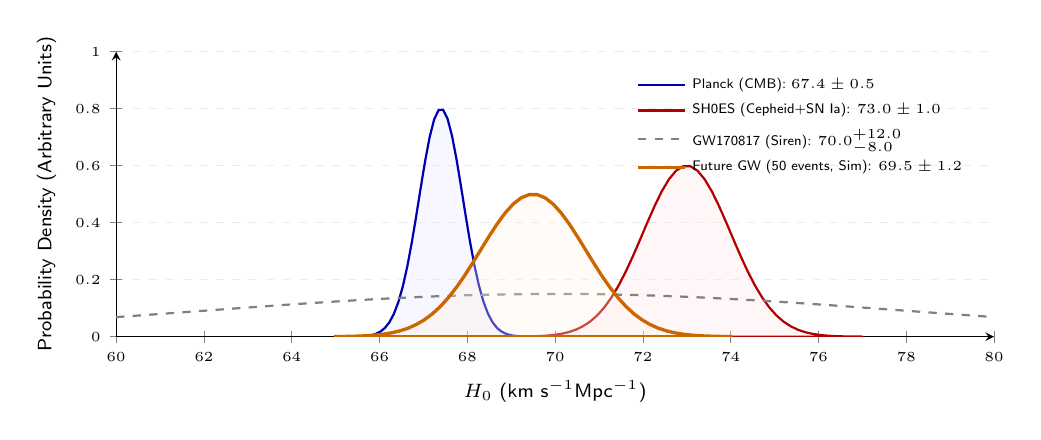
\begin{tikzpicture}
        \begin{axis}[
          width=1.05\textwidth,
          height=5.2cm,
          xmin=60, xmax=80,
          ymin=0, ymax=1.0,
          xlabel={$H_0$ ($\text{km s}^{-1}\text{Mpc}^{-1}$)},
          ylabel={Probability Density (Arbitrary Units)},
          axis x line=bottom,
          axis y line=left,
          enlargelimits=false,
          ymajorgrids=true,
          grid style={color=gray!15, dashed},
          tick label style={font=\tiny},
          label style={font=\scriptsize},
          legend style={at={(0.98,0.95)}, anchor=north east, font=\fontsize{4pt}{5pt}\selectfont, draw=none, fill=none},
          legend cell align={left}
        ]
          % Planck (Early)
          \addplot[
            color=blue!70!black,
            thick,
            domain=65:70,
            samples=50,
            fill=blue!10,
            fill opacity=0.3
          ] {0.8 * exp(-0.5*((x-67.4)/0.5)^2)} \closedcycle;
          \addlegendentry{Planck (CMB): $67.4 \pm 0.5$}
      
          % SH0ES (Late)
          \addplot[
            color=red!70!black,
            thick,
            domain=69:77,
            samples=50,
            fill=red!10,
            fill opacity=0.3
          ] {0.6 * exp(-0.5*((x-73.0)/1.0)^2)} \closedcycle;
          \addlegendentry{SH0ES (Cepheid+SN Ia): $73.0 \pm 1.0$}
      
          % GW170817
          \addplot[
            color=black!50,
            thick,
            dashed,
            domain=60:80,
            samples=50
          ] {0.15 * exp(-0.5*((x-70.0)/8.0)^2)};
          \addlegendentry{GW170817 (Siren): $70.0^{+12.0}_{-8.0}$}
          
          % Future GW
          \addplot[
            color=orange!80!black,
            very thick,
            domain=65:74,
            samples=50,
            fill=orange!10,
            fill opacity=0.3
          ] {0.5 * exp(-0.5*((x-69.5)/1.2)^2)} \closedcycle;
          \addlegendentry{Future GW (50 events, Sim): $69.5 \pm 1.2$}
        \end{axis}
      \end{tikzpicture}
    \end{column}
  \end{columns}
\end{frame}

% Slide 6: Results Slide with Table
\begin{frame}{Comparison of Cosmological Probes}{Summary of Current H0 Measurements}
  \centering
  \begin{table}
    \caption{Key measurements of the Hubble constant $H_0$ across different methods.}
    \vspace{0.2em}
    \fontsize{8.5pt}{10.5pt}\selectfont
    \begin{tabular}{llcl}
      \toprule
      \textbf{Method} & \textbf{Probe / Catalog} & \textbf{$H_0$ Value (km s$^{-1}$Mpc$^{-1}$)} & \textbf{Reference} \\
      \midrule
      Early Universe & Planck CMB & $67.4 \pm 0.5$ & Planck Collab. (2020) \\
      Local Ladder & SH0ES (Cepheids) & $73.0 \pm 1.0$ & Riess et al. (2022) \\
      TRGB & CCHP (TRGB) & $69.8 \pm 0.8$ & Freedman et al. (2021) \\
      Strong Lensing & H0LiCOW & $73.3^{+1.7}_{-1.8}$ & Wong et al. (2020) \\
      \midrule
      \textbf{Standard Sirens} & \textbf{GW170817 (Siren)} & \textbf{$70.0^{+12.0}_{-8.0}$} & \textbf{Abbott et al. (2017)} \\
      \bottomrule
    \end{tabular}
  \end{table}
  \begin{minipage}{0.9\textwidth}
    \centering
    \fontsize{8pt}{10pt}\selectfont\color{cosmicslate} Note: Standard sirens represent the only probe capable of a direct, self-calibrated distance measurement at cosmological distances without the need for a local distance ladder.
  \end{minipage}
\end{frame}

% Slide 7: Conclusions Slide
\begin{frame}{Conclusions \& Takeaways}
  \begin{itemize}
    \item \textbf{The Hubble Tension remains robust} at $\sim 5\sigma$ between CMB measurements ($67.4 \pm 0.5$) and local distance ladder measurements ($73.0 \pm 1.0$).
    \vspace{0.8em}
    \item \textbf{Standard Sirens offer a clean, independent path} to arbitrate this tension, relying on general relativity for absolute distance calibration.
    \vspace{0.8em}
    \item \textbf{A single event (GW170817) demonstrated the proof of concept}, establishing $H_0 \approx 70^{+12}_{-8} \text{ km s}^{-1}\text{Mpc}^{-1}$.
    \vspace{0.8em}
    \item \textbf{Next-generation catalogs (LVK O4/O5) will provide $\sim 50$ events}, yielding a $1.5\%$ measurement of $H_0$, which will decisively test cosmological models.
  \end{itemize}
\end{frame}

% Slide 8: Closing thank-you slide
\begin{frame}[plain,c]
  \centering
  \vfill
  {\color{cosmicgold}\rule{2cm}{1.5pt}}\par\vspace{0.6cm}
  {\usebeamerfont{section title}\color{cosmicnavy}\bfseries Thank You}\par
  \vspace{0.4cm}
  {\color{cosmicslate}\large Questions \& Comments}\par
  \vspace{1.5cm}
  {\fontsize{8pt}{10pt}\selectfont\color{cosmicslate} Email: elena.vance@igp.edu \quad | \quad Web: igp.edu/evance}
  \vfill
\end{frame}

\end{document}
